\subsection{Kapitel 4}
Eva wurde schwanger und gebar den Kain\footnote{bed. Erwerb}. Später gebar sie einen zweiten Sohn mit dem Namen Abel. Ich glaube das ist das berühmteste Pärchen auf dieser Welt. Kain und Abel. Es heisst hier, Kain war Ackerbauer und Abel ein Schafhirte. Beide brachten dem Herrn ein Opfer dar. Kain von den Früchten der Erde und Abel schlachtete ein Schaf. Gott sah das Opfer von Abel an aber das von Kain nicht. War es wirklich nur darum, dass Kain kein Tier geschlachtet hat? Ich kann das nichst so recht glauben. Kann es nicht auch sein, dass Kain schon immer ein Problemkind war? Als Gott sein Opfer nicht anerkannte, wurde er ja ziemlich zornig auf seinen Bruder. Wenn ich ohne Gott unterwegs bin und gegen ihn sündige, wird es wohl nicht reichen wenn ich ihm einfach ein Opfer darbringe und denke, jetzt ist er wieder zufrieden mit mir. Als er dann sah dass es doch nicht so einfach ist Gott zu beeinflussen, wurde er dann halt sauer. Gott ihn ja darauf aufmerksam gemacht. Er hätte es vor Gott wieder gutmachen können.
\begin{bibeltext}{ELB}{Gen}{4:6-7}
	Und der \herr{} sprach zu Kain: "Warum bist du ergrimmt, und warum und warum hat sich dein Angesicht gesent? Ist es nicht so, dass es sich erhebt, wenn du recht tust?"
\end{bibeltext}
Das ist doch etwas was uns auch immer wieder passiert. Wenn wir merken, dass wir etwas schlimmes getan haben, ducken wir uns und wir dürfen nicht mehr direkt in die Augen schauen? Da gibt es dann Zwei Möglichkeiten, wir biegen das geleistete wieder gerade und bringen es vor Gott oder wir kehren es unter den Tisch und warten bis sich alles als Hass in uns aufgestaut hat. Man wird bitter und wird böse gegenüber der Umwelt. Wer jetzt eher Gewalttätig ist lässt es an anderen raus oder er tut sich selber Gewalt an. Kain ging dann in die grosse weite Welt und gründete dort eine Stadt. Die Nachkommen Kain gründeten die Zivilisation. Adam bekam noch einen weiteren Sohn. Diese Sohn nannte er Set. Aus der Linie Set entstammte Noah.
\subsection{Kapitel 5}
\begin{figure}[ht]
	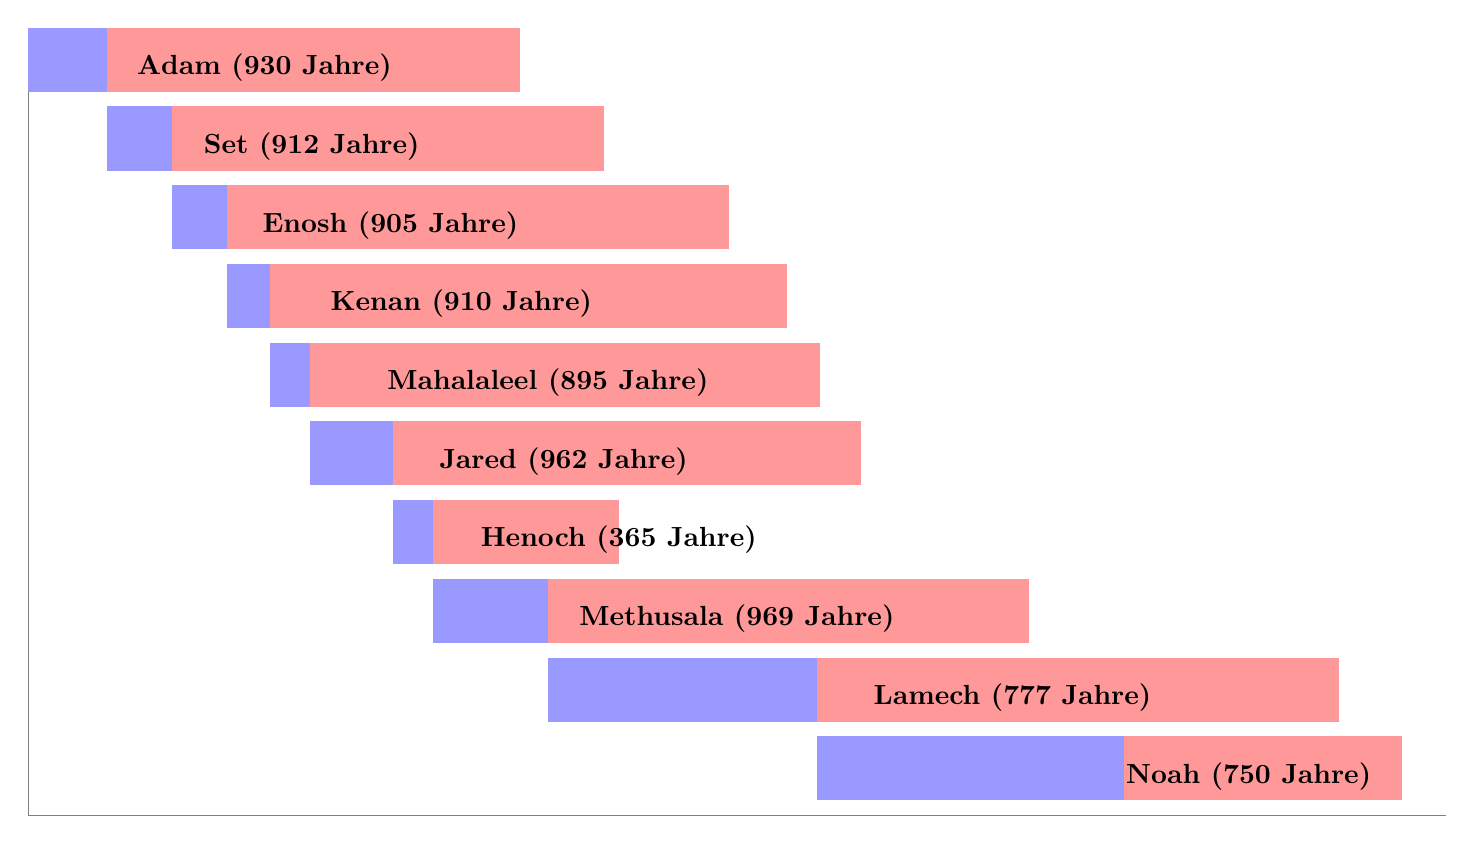
\begin{tikzpicture}
		\draw[gray] (0,0) -- (0mm, 100mm);
		%Adam 130-800 (10.1 - 62.4)
		\filldraw[blue!40] (0,100mm) rectangle(10.1mm,92mm);
		\filldraw[red!40] (10.1mm,100mm) rectangle(62.4mm,92mm) node at (30mm, 92mm) [right, above, black]{\textbf{Adam (930 Jahre)}};
		%Set 105-807 (8.19 - 62.9)
		\filldraw[blue!40] (10.1mm,90mm) rectangle(18.29mm,82mm);
		\filldraw[red!40] (18.29mm,90mm) rectangle(73.0mm,82mm) node at (36mm, 82mm) [right, above, black]{\textbf{Set (912 Jahre)}};
		%Enosch 90 - 815 (7.02 - 63.6)	
		\filldraw[blue!40] (18.29mm,80mm) rectangle (25.31mm,72mm);
		\filldraw[red!40] (25.31mm,80mm) rectangle(88.91mm,72mm) node at (46mm, 72mm) [right, above, black]{\textbf{Enosh (905 Jahre)}};
		%Kenan 70 - 840 (5.46 - 65.52)		
		\filldraw[blue!40] (25.31mm,70mm) rectangle(30.77mm,62mm);
		\filldraw[red!40] (30.77mm,70mm) rectangle(96.29mm,62mm) node at (55mm, 62mm) [right, above, black]{\textbf{Kenan (910 Jahre)}};
		%Mahalaleel 65 - 830 (5.07 - 64.7)
		\filldraw[blue!40] (30.77mm,60mm) rectangle(35.84mm,52mm);
		\filldraw[red!40] (35.84mm,60mm) rectangle(100.54mm,52mm) node at (66mm, 52mm) [right, above, black]{\textbf{Mahalaleel (895 Jahre)}};
		%Jared 162 - 800 (12.6 - 62.4)
		\filldraw[blue!40] (35.84mm,50mm) rectangle(46.44mm,42mm);
		\filldraw[red!40] (46.44mm,50mm) rectangle(105.68mm,42mm) node at (68mm, 42mm) [right, above, black]{\textbf{Jared (962 Jahre)}};
		%Henoch 65 - 300 (5.07 - 23.4)
		\filldraw[blue!40] (46.44mm,40mm) rectangle(51.51mm,32mm);
		\filldraw[red!40] (51.51mm,40mm) rectangle(74.91mm,32mm) node at (75mm, 32mm) [right, above, black]{\textbf{Henoch (365 Jahre)}};
		%Methusalah 187 - 782 (14.58 - 60.99)
		\filldraw[blue!40] (51.51mm,30mm) rectangle(66.09mm,22mm);
		\filldraw[red!40] (66.09mm,30mm) rectangle(127.08mm,22mm) node at (90mm, 22mm) [right, above, black]{\textbf{Methusala (969 Jahre)}};
		%Lamech 182 - 595 (14.19 - 46.41)
		\filldraw[blue!40] (66.09mm,20mm) rectangle(100.28mm,12mm);
		\filldraw[red!40] (100.28mm,20mm) rectangle(166.37mm,12mm) node at (125mm, 12mm) [right, above, black]{\textbf{Lamech (777 Jahre)}};
		% Noah 500 - 450 (39 - 35.1)
		\filldraw[blue!40] (100.28mm,10mm) rectangle(139.28mm,2mm);
		\filldraw[red!40] (139.28mm,10mm) rectangle(174.38mm,2mm) node at (155mm, 2mm) [right, above, black]{\textbf{Noah (750 Jahre)}};

		\draw[gray] (0,0) -- (180mm, 0mm);
	\end{tikzpicture}
	\caption{Lebensjahre bis Noah}
	\label{balken_alter}
\end{figure}
In diesem Kapitel wird das Geschlechtsregister Adams bis Noah aufgelistet. Die Menschen wurden zu der Zeit ziemlich alt. Durch dieses Alter gab es eine Spezielle konstellation.
Es ist interessant zu sehen (Abbildung: \ref{balken_alter}), wie Noah noch die Geburt von Lamech knapp miterleben konnte. Ich glaube zwar nicht, dass die sich nach so langer Zeit noch gekannt haben, aber es ist spannend. Am Ende das blauen Balken wurde dann der erste Sohn geboren, oder wenigsten die Person die die direkte Linie zu Jesus weiter führte.
Dieses Kapitel endet mit der Erwähnung von Noah und es werden seine Söhne Sem, Ham, Japhet aufgelistet.
